Every piece of software should be written in a way that is testable. Moreover it is really important for framework to have tests. There are many ways to test software. Two main categories emerged when dealing with this problem. Manual, which comes down to compile, run and observe behaviour and if it matches your expectations then proceed with testing of another functionality. Automatic, there are many approaches here. The one that was performed for the purpose of this work is called ``unit testing''.

It is also necessary to check that created solution actually works on a real system. Some testing environment was created in order to utilize the full capabilities of provided features and will be discussed later on in this chapter.

\section{Unit testing}
Which is also called testing in separation. What does it really mean is the fact that we only check the correctness of logic of only one particular function. Those should have at least $2^n$ unit tests where $n$ is number of branches in function body (e.g.\ ifs blocks). Every dependencies and calls to others functions have to be ``mocked''. Mocking is a technique of injecting exactly the same signature of mocked function, yet with predefined behaviour like fixed return value.

Unit testing is also specific to language of written application. In Go there is a special package \verb|testing| which provides methods to mark tests as failed.

Every file which contains unit tests must be suffixed with \verb|_test| in file name\cite{Testing-go} in order for command \verb|go test| to be able to discover where unit tests are. In addition every function must be prefixed with \verb|Test| keyword and have one argument \verb|*testing T|, because aforementioned tool for executing test will call every test function with that argument.

In body of unit test function we check the behaviour of function by calling it and comparing with expected result. Therefore it is a common pattern to called those variables ``actual'' and ``expected'. If those two are not the same then we will call method \verb|Error| or similar on \verb|*testing T| to mark the test as failed.

Go standard library defines also very handy package \verb|httptest|\cite{httptest-go} that have exactly the same signatures and interfaces as a package \verb|http|, yet no actual data is being send over http protocol, but the actual calls could be further inspected which is crucial in order to maintain logic separation.

Recall simple middleware (\ref{src:example-middleware}) for setting \verb|Content-Type| to JSON\@. The expected value of  \verb|Content-Type| is stored in \verb|expected| variable. Then we manually set up wrong header, then recorder is being created. \verb|HTTPHandlerMock| has the same interface as \verb|HTTPHandler| so it can be used as mock. Tested function is then called with mocked arguments, \verb|ServeHTTP| will spin up the faked server. Variable \verb|header| represents the actual data that is further compared to expected value. If condition is not met then message from method \verb|Errorf| will be printed to the console and command \verb|go test| will exit with non-zero status code.

\begin{figure}[!htbp]
\begin{verbatim}
func TestSetJSONHeader(t *testing.T) {
        expected := "application/json; charset=utf-8"

        r, _ := http.NewRequest("GET", "", nil)
        r.Header.Set("Content-Type", "application/x-www-form-urlencoded")

        w := httptest.NewRecorder()

        mock := &HTTPHandlerMock{w, r}
        handler := SetJSONHeader(mock)

        handler.ServeHTTP(mock.w, r)

        header := mock.w.Header().Get("Content-Type")
        if header != expected {
                t.Errorf("Expected %s, got `%s`", expected, header)
        }
}
\end{verbatim}
\renewcommand\figurename{Code}
\caption{Unit test of example middleware that sets response headers}
\label{src:test-example-middleware}
\end{figure}

\section{Testing environment}
Every software after being implemented needs to be tested on some set up. For the purpose of this framework I wrote simple application that utilizes features of the framework.

\begin{figure}[!htbp]
\centering
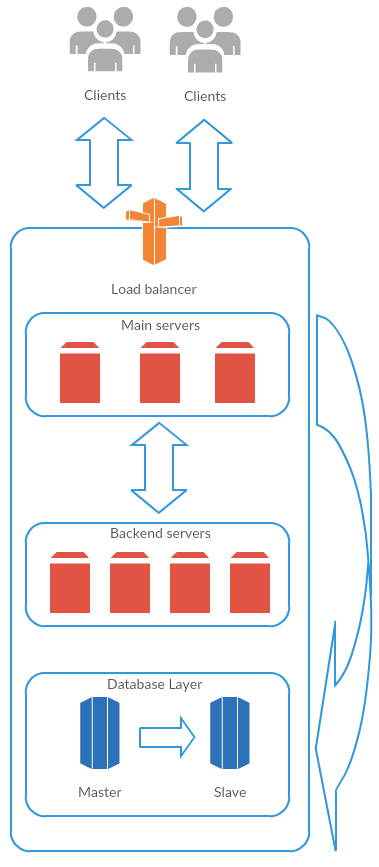
\includegraphics[scale=1.0]{architecture}
\label{fig:architecture}
\caption{Architecture of the whole system}
\end{figure}

Architecture contains main server which serves data to clients (in this case users equipped with web browsers). Then it communicate with backend servers through RESTful API to get data for clients.

In addition main server is an entity which can represent multiple servers hidden behind load balancer for scaling for high load plus one additional server for storing database and shared files via NFS\@.

Created application had three resources exposed on URIs, all communication was held by exchanging JSON objects in body of a request. Everything was exposed on IP 10.0.0.2 on port 80.
\begin{itemize}
    \item \verb|/user|
    \begin{itemize}
        \item \verb|POST| --- creates new user, required fields \verb|user_name|, \verb|password|
        \item \verb|PUT| --- updates the user details, required fields \verb|user_name|, \verb|password|, the user needs to be authenticated in order to use this verb
        \item \verb|DELETE| --- removes the user itself, the user needs to be authenticated in order to use this verb
    \end{itemize}
    \item \verb|/login|
    \begin{itemize}
        \item \verb|POST| --- authenticate user, required fields \verb|user_name|, \verb|password|
    \end{itemize}
    \item \verb|/hello|
    \begin{itemize}
        \item \verb|GET| --- greets the user using its \verb|user_name| field, the user needs to be authenticated in order to use this verb
    \end{itemize}
\end{itemize}

I used famous program \verb|curl| in order to interact with REST API created from the framework.

First, let us register
\begin{verbatim}
curl -H "Content-Type: application/json "
    -d '{"user_name": "test", "password": "testpw"}' \
    http://10.0.0.2/user -v
\end{verbatim}

This time I added \verb|-v| switch which will show us how request was made and was the response was in more detail.
\begin{verbatim}
*   Trying 10.0.0.2...
* Connected to TEST-SERVER (10.0.0.2) port 80 (#0)
> POST /user HTTP/1.1
> Host: 10.0.0.2:80
> User-Agent: curl/7.43.0
> Accept: */*
> Content-Type: application/json
> Content-Length: 43
* upload completely sent off: 43 out of 43 bytes
< HTTP/1.1 200 OK
< Date: Sun, 13 Mar 2016 15:57:56 GMT
< Content-Length: 9
< Content-Type: application/json; charset=utf-8
* Connection #0 to host TEST-SERVER left intact
\end{verbatim}

Server responded with with status code 200, which means everything went smooth. One more thing to notice is the fact that simple middleware which set proper Content-Type works perfectly. We can now login. For further tests the \verb|-v| switch will be omitted as well as header which sets Content-Type for simplicity.

\begin{verbatim}
curl -d '{"user_name": "test", "password": "testpw"}' \
    http://10.0.0.2/login

{"token": "eyJhbGciOiJIUzI1NiIsInR5cCI6IkpXVCJ9.
eyJ1c2VyX25hbWUiOiJ0ZXN0In0.
XK4_cM7j8tCzcDRRM4iYNqeoyDQtPmNouhR_ITlj8JE"
\end{verbatim}

As expected this time, server responded with base64 encoded token. I used website \url{jwt.io} to confirm that token was generated properly and the signature can be verified. If we want to make an request to resource which requires authentication, we need to put this token into \verb|Authentication| field in request header, like
\begin{verbatim}
curl -H "Authentication: token" http://10.0.0.2/user
\end{verbatim}

So let us make a authentication request to \verb|/hello|.
\begin{verbatim}
curl -H "Authentication: eyJhbGciOiJIUzI1NiIsInR5cCI6IkpXVCJ9. \
    eyJ1c2VyX25hbWUiOiJ0ZXN0In0. \
    XK4_cM7j8tCzcDRRM4iYNqeoyDQtPmNouhR_ITlj8JE" \
    http://10.0.0.2/hello

{"msg": "Hello test"}
\end{verbatim}

Server responded with a string ``Hello'' plus our \verb|user_name| which was \verb|test|. Finally let us try to remove the account (recall that the request needs to be authenticated).
\begin{verbatim}
curl -H "Authentication: token" -X DELETE http://10.0.0.2/user
\end{verbatim}

The server responded with 200 again, with no additional message which indicates that out account should be removed. But it needs to verified.
\begin{verbatim}
curl -d '{"user_name": "test", "password": "testpw"}' \
    http://10.0.0.2/login
\end{verbatim}

This time returned message was 401 Unauthorized. It clearly states that the authentication failed, because the user no longer exists in a database.
